\chapter{KV-Cache Infrastructure Techniques}\label{chapter:techniques}

This chapter reviews techniques for representing and compressing the KV-cache, organizing its storage and access, and managing its reuse across executions. We use the three challenges introduced in Chapter~\ref{chapter:background} to explain the benefits and costs of these designs.

\section{Representation and Compression}\label{sec:techniques:representation}

Representation and compression techniques reduce the data volume of KV-cache that must be retained for attention. Equation~\ref{eq:background:capacity} suggests three broad approaches: reduce the number or dimensions of independent key-value representations, retain fewer historical entries, or use fewer bits for each value. We organize this section accordingly into structural compression, selective retention, and numerical quantization. The distinction concerns what is compressed; a system may combine several approaches.

\subsection{Model Structural-Based Reduction}\label{sec:techniques:structural}

The model structure changes how keys and values are represented across heads, layers, or vector dimensions. Some methods introduce an attention architecture that produces a smaller cache from the outset. Others transform an existing model to use a more compact representation. This distinction matters because an architectural change may require training, whereas a transformation of an existing model must control the error introduced by compression.

\begin{figure}[h]
    \centering
    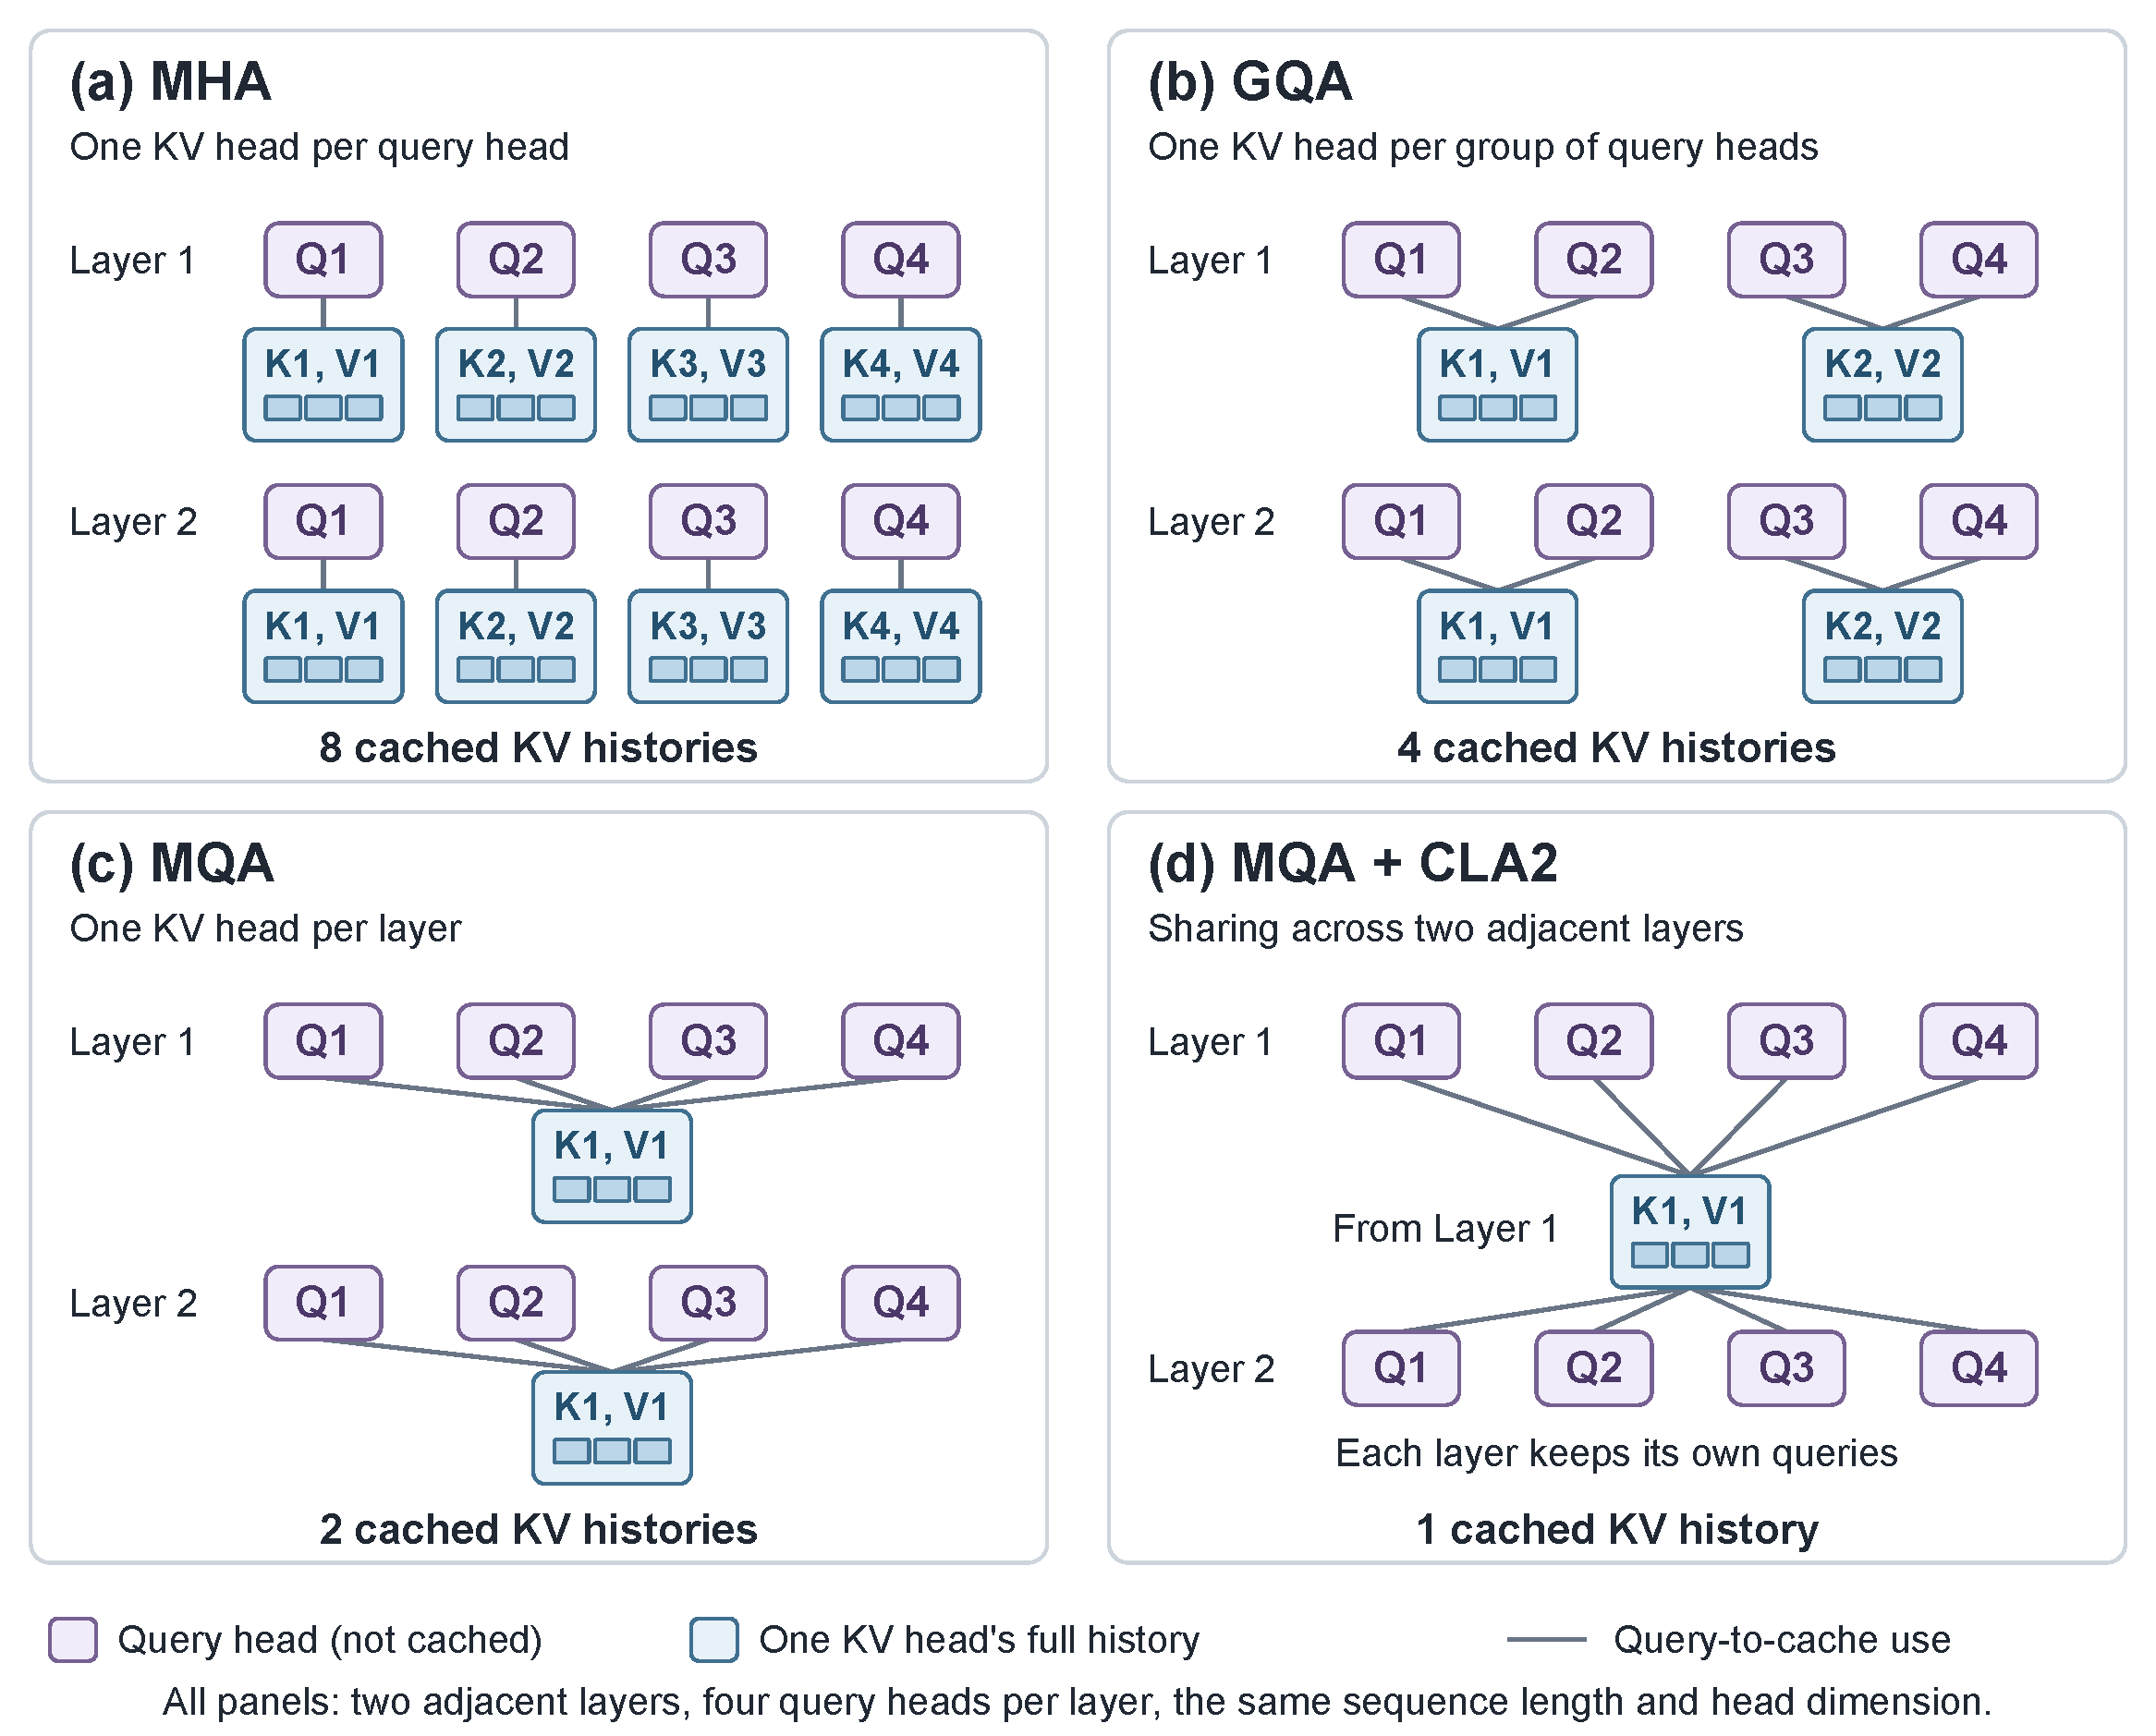
\includegraphics[width=0.8\textwidth]{figures/attention-cache-sharing.pdf}
    \caption{KV-cache sharing across heads and layers.}
    \label{fig:kv-sharing}
\end{figure}

\paragraph{Sharing across heads and layers.}
In conventional multi-head attention (MHA), each head uses separate projections to generate queries, keys, and values. Each head therefore requires its own cached keys and values for all retained token positions. The cache size grows with the number of heads as well as the sequence length.

Grouped-query attention (GQA) divides query heads into groups, with each group sharing one key-value head~\cite{kv_ainslie2023gqa}. Multi-query attention (MQA), introduced to reduce decoding bandwidth demand, is the special case with only one group~\cite{kv_shazeer2019mqa}. GQA reduces cached vectors without reducing the number of query heads. This distinction helps explain why sharing can preserve model quality: distinct queries can assign different attention weights to the same keys and extract different weighted combinations of the shared values. Keeping several KV groups also preserves more representational diversity than MQA. To adapt an existing MHA checkpoint, the authors average the key and value projection weights within each group and continue training. This allows the model to adjust to sharing, achieving quality close to MHA in their experiments. Quality preservation is therefore an empirical outcome of the sharing configuration and adaptation, rather than a guarantee of lossless compression.

Cross-Layer Attention (CLA) extends sharing to adjacent layers~\cite{kv_brandon2024cla}. In its pairwise configuration, the first layer generates keys and values that both layers use, halving the number of separately cached layers. The second layer still generates its own queries from its updated hidden states and retains its own output projection and feed-forward network. Mechanistically, this allows successive layers to extract different information from a common cache and continue transforming it; sharing KV does not require identical attention outputs or merging whole layers. Training with this architecture lets the shared representation serve both layers. The paper's experiments show that pairwise sharing can retain nearly the same accuracy as MQA while reducing its cache size. This is evidence that separately generated KV representations are not essential at every layer in the tested models, rather than proof that neighboring layers' KV tensors in an arbitrary pretrained model are already interchangeable.

MiniCache uses cross-layer similarity without retraining the model~\cite{kv_liu2024minicache}. It merges similar KV vectors from adjacent middle-to-deep layers by interpolating their directions while retaining their magnitudes, and keeps sufficiently different entries separate. Whereas CLA learns a shared representation through its architecture, MiniCache approximates representations already produced by a model. Its capacity benefit therefore depends on the observed similarity and the fraction of entries that remain unmerged.

\paragraph{Using fewer dimensions.}
Multi-head Latent Attention (MLA), introduced in DeepSeek-V2, instead builds a compact representation into the model architecture~\cite{kv_deepseek2024v2}. It generates a shared latent vector---a smaller learned representation---from which multiple key and value heads are defined. During decoding, transformations can be combined with the query and output projections to avoid explicitly reconstructing all historical keys and values. MLA also separates the positional component of attention and retains an additional positional key. Its cache therefore contains both the latent vectors and this positional information. MLA is learned as part of the model architecture.

These methods primarily address capacity pressure. They can also reduce access bandwidth pressure when the attention implementation consumes shared or reduced representations efficiently. However, a smaller stored cache does not imply a proportional reduction in memory traffic: shared data may still be read by multiple operations. Architectural adaptation, approximation error, and support in the attention implementation determine whether a structural reduction becomes a practical serving benefit.

\begin{figure}[h]
    \centering
    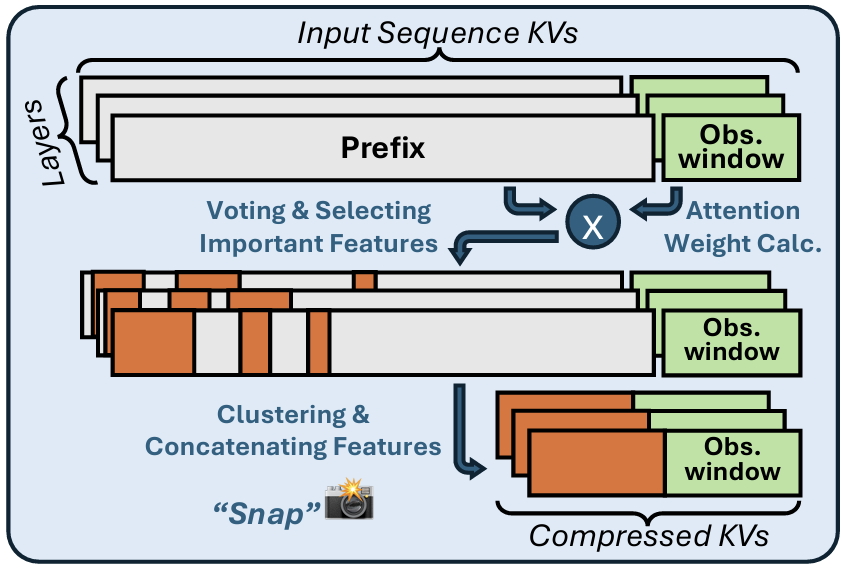
\includegraphics[width=0.45\textwidth]{figures/kv-selection.png}
    \caption{KV-cache selection.}
    \label{fig:kv-selection}
\end{figure}

\subsection{Selective Retention}\label{sec:techniques:retention}

Selective retention reduces the historical information kept for an active sequence. A cache budget specifies how many entries may remain, and a selection policy determines which entries to retain as the sequence grows. The main design choices are how importance is estimated, how the budget is distributed across heads and layers, and when the selection is updated.

\paragraph{Retention by observed importance.}
H$_2$O uses observed attention to select useful historical entries~\cite{kv_zhang2023h2o}. It combines recent tokens with \emph{heavy hitters}, tokens that have accumulated large attention scores. As generation proceeds, the system updates these statistics and removes lower-priority entries to respect the cache budget. Compared with a fixed positional rule, this can preserve older information that continues to receive attention. The cost is maintaining importance scores and performing selection during inference. Moreover, accumulated attention reflects past queries, so it cannot guarantee that an evicted token will remain irrelevant to future queries.

SnapKV moves the selection of historical prompt entries to the end of prefill~\cite{kv_li2024snapkv}. It observes attention from a short window at the end of the prompt to estimate which earlier positions each head will need during generation. It pools importance scores over neighboring positions, selects entries for each head, and retains the observation window. The resulting prompt cache is smaller before decoding begins. This reduces the need to repeatedly select among all prompt entries, but relies on the prompt's final attention pattern being informative about subsequent generation. Selecting the prompt cache also does not, by itself, impose a fixed bound on all entries added during a long output.

\paragraph{Distributing the retention budget.}
Choosing which entries to retain is separate from deciding how much capacity each layer receives. PyramidKV observes that attention in its studied models is more broadly distributed in lower layers and more concentrated in higher layers~\cite{kv_cai2025pyramidkv}. It assigns larger budgets to lower layers and smaller budgets to higher layers, while selecting important positions within the heads. The allocation reflects an observed pattern rather than a universal property of attention; its suitability depends on the model and workload.

Selective retention can relieve both capacity pressure and access bandwidth pressure because fewer entries remain for subsequent attention. Its principal trade-off is loss of historical information, together with the cost of computing and maintaining selection decisions. These costs occur at different times: prompt selection adds work during state preparation, while an online eviction policy adds work during generation. If discarded information is needed again, restoring it may require recomputation from the original context. The useful comparison is therefore between the retained information, the timing of selection, and the demands of the target task, rather than cache size alone.

\subsection{Numerical Quantization}\label{sec:techniques:quantization}

Quantization stores numerical values using a smaller set of representable values, reducing the bits needed per cache element. Unlike token eviction, it can retain entries for every historical position, but approximates their contents. Its effectiveness depends on which values share quantization parameters, how unusual values are handled, and how the compressed representation participates in attention.

KIVI uses different quantization rules for keys and values~\cite{kv_liu2024kivi}. A \emph{channel} is one dimension of a key or value vector; a quantization group contains numbers that share quantization parameters. For keys, KIVI groups numbers from the same channel across tokens. Large key magnitudes often concentrate in particular channels, so this prevents them from reducing precision in other channels. For values, it groups numbers within each token's vector, limiting the influence of one token's extreme values on other tokens. KIVI keeps recent entries at higher precision and quantizes older entries in fixed-size groups, since key quantization requires accumulating multiple tokens. The cache therefore contains both low-precision groups and a higher-precision recent portion, rather than storing every entry in two bits.

Coupled Quantization (CQ) divides each key vector and each value vector separately into small, non-overlapping groups of consecutive components~\cite{kv_zhang2024cq}. Across tokens, components within a group exhibit statistical dependencies: some combinations of values occur more often than others. CQ learns a collection of representative vectors, called a \emph{codebook}, for each group and stores only the index of the representative that approximates its components together. Keys and values are not combined into one group. One index thus encodes several components. Codebooks are learned from sample inputs, accounting for how quantization errors affect model outputs. This approach requires codebook storage, work to select representative vectors, and specialized attention computation.

Quantization directly reduces capacity demand and can reduce the bytes transferred during cache access. Whether it improves generation speed depends on how KV-cache are decoded and consumed. \emph{Dequantization} converts a compressed representation back to forms usable by the computation. The extra writes, reads, and temporary storage during dequantization can offset compression benefits.  Numerical error, metadata, higher-precision exceptions, and conversion work must therefore be considered alongside nominal bit width.

\subsection{Comparison and Composability}\label{sec:techniques:compression-summary}

Table~\ref{tab:compression-comparison} summarizes the main distinctions among the reviewed methods. Architectural methods change which representations a model produces; selective retention changes which historical entries survive; quantization changes how retained values are encoded.

\begin{table}[t]
    \centering
    \caption{Representative compression methods and their design trade-offs. Calibration configures a method using sample inputs; it need not involve updating the model through training.}
    \label{tab:compression-comparison}
    \begingroup
    \footnotesize
    \setlength{\tabcolsep}{4pt}
    \renewcommand{\arraystretch}{1.15}
    \begin{tabularx}{\textwidth}{@{}>{\raggedright\arraybackslash}p{0.18\textwidth}>{\raggedright\arraybackslash}p{0.23\textwidth}>{\raggedright\arraybackslash}p{0.23\textwidth}>{\raggedright\arraybackslash}X@{}}
        \toprule
        \textbf{Method} & \textbf{Main change} & \textbf{Preparation or adaptation} & \textbf{Main cost or limitation} \\
        \midrule
        GQA~\cite{kv_ainslie2023gqa} & Share KV heads & Training or checkpoint adaptation & Fewer independent KV heads \\
        CLA~\cite{kv_brandon2024cla} & Share KV across layers & Architectural training & Dependencies between layers \\
        MiniCache~\cite{kv_liu2024minicache} & Merge similar adjacent-layer KV & No retraining & Approximation; unmerged exceptions \\
        MLA~\cite{kv_deepseek2024v2} & Cache a latent representation & Architectural training & Specialized attention computation \\
        \addlinespace[4pt]
        H$_2$O~\cite{kv_zhang2023h2o} & Keep recent and high-score tokens & Online score updates & Selection cost; future relevance uncertain \\
        SnapKV~\cite{kv_li2024snapkv} & Select prompt entries per head & Attention observation at prefill & Depends on observed prompt attention \\
        PyramidKV~\cite{kv_cai2025pyramidkv} & Vary retention budgets by layer & Layer budget configuration & Assumes suitable attention patterns \\
        \addlinespace[4pt]
        KIVI~\cite{kv_liu2024kivi} & Quantize keys and values differently & Online grouped quantization & Numerical error; residual cache \\
        CQ~\cite{kv_zhang2024cq} & Encode channels jointly & Codebook calibration & Codebook storage and lookup \\
        \bottomrule
    \end{tabularx}
    \endgroup
\end{table}

The approaches can be complementary: a model with shared KV heads may retain selected token positions and quantize the remaining values. Compatibility is nevertheless a design question. A selection policy must respect any sharing of the underlying entries; a quantizer calibrated for full-dimensional keys may need to be adapted to latent vectors. Errors from selection, dimensional reduction, and quantization can also interact.

Across the three bottlenecks, compression most directly targets capacity and access bandwidth. A smaller representation may also reduce transfer or loading time when cached data is reused, while encoding, selection, or restoration may add state preparation work. This motivates treating representation as one part of the infrastructure: the storage system must support the chosen format, and reuse policies must account for what information the compressed cache still contains.

\section{Storage and Access}\label{sec:techniques:storage}

Storage and access techniques determine how KV-cache entries occupy physical memory and reach attention computation. We review allocation and address mapping together with their support for attention, followed by storage across devices. These mechanisms support a chosen cache representation; identifying reusable contexts and coordinating their consumers are separate responsibilities.

\begin{figure}[h]
    \centering
    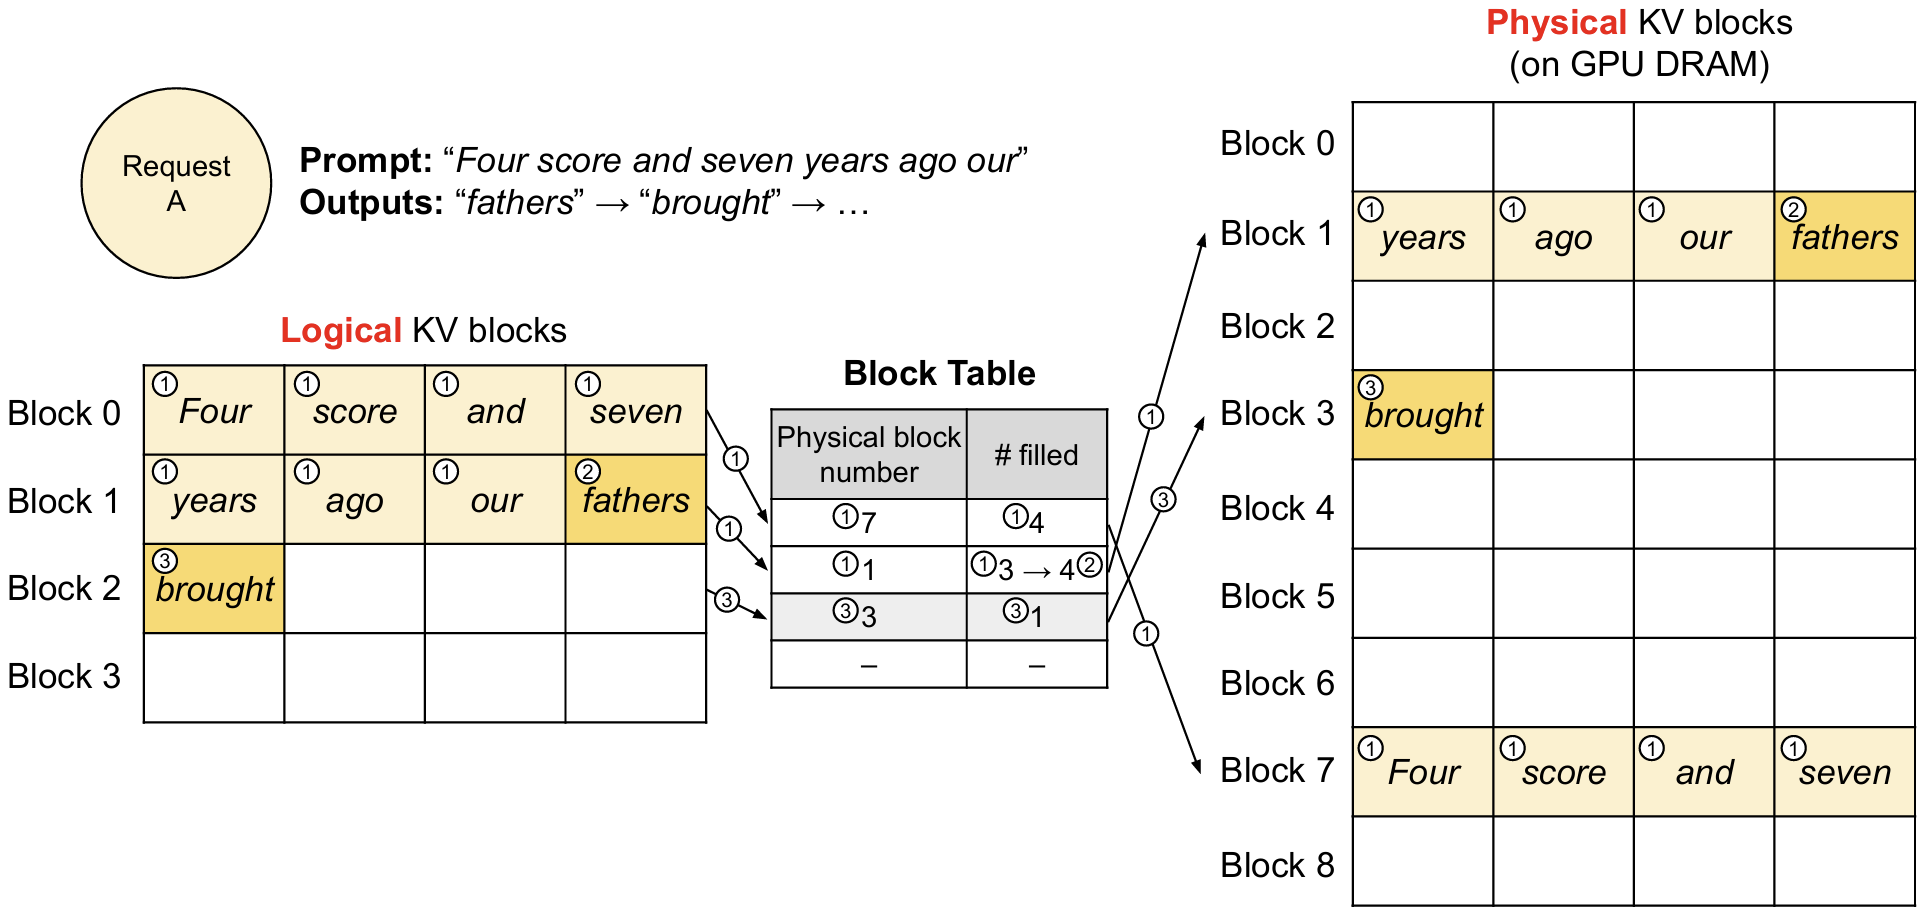
\includegraphics[width=0.95\textwidth]{figures/page-mapping.png}
    \caption{PagedAttention and vAttention divide the KV-cache of a sequence into fixed-sized blocks (pages) and manage them in discrete physical memory slots.}
    \label{fig:page-mapping}
\end{figure}

\subsection{Allocation and Address Mapping}\label{sec:techniques:allocation}

Sequences grow during decoding and have different lengths. Reserving a large contiguous region for each sequence wastes unused space, while repeatedly enlarging an allocation may require copying existing entries. Dynamic allocation must therefore accommodate growth without excessive reservation or movement.

PagedAttention~\cite{kv_kwon2023pagedattention} allocates fixed-size cache blocks as a sequence grows. A block table maps positions in the sequence to blocks in GPU memory, allowing attention to read physically scattered data. This reduces wasted capacity, although the final block may remain partially unused. The cost is maintaining mappings and adapting attention implementations to follow them. Multiple sequences can also reference the same physical blocks; deciding which contexts qualify for sharing is a separate reuse problem.

vAttention instead preserves contiguous \emph{virtual addresses}, the addresses used by the program, while allocating the underlying physical memory on demand~\cite{kv_prabhu2025vattention}. It uses GPU virtual-memory support to separate these two views, allowing existing attention implementations to retain contiguous access. Both approaches relieve capacity pressure; their main distinction is whether address mapping is handled explicitly by the attention implementation or through the virtual-memory system. The latter still requires managing allocation and mapping costs.

\paragraph{Supporting attention computation.}
Attention routines must support the cache layout. For example, an implementation requiring contiguous data would need scattered cache blocks copied into a temporary buffer, adding memory traffic and space. PagedAttention avoids this copy by reading through block mappings. FlashInfer supports different organizations, including paged and shared-prefix caches, through a common block-based representation and corresponding GPU attention routines~\cite{kv_ye2025flashinfer}. These routines access the stored blocks directly, but must be compatible with the chosen layout. Efficient allocation therefore needs matching attention support to avoid additional access costs.

\begin{figure}[h]
    \centering
    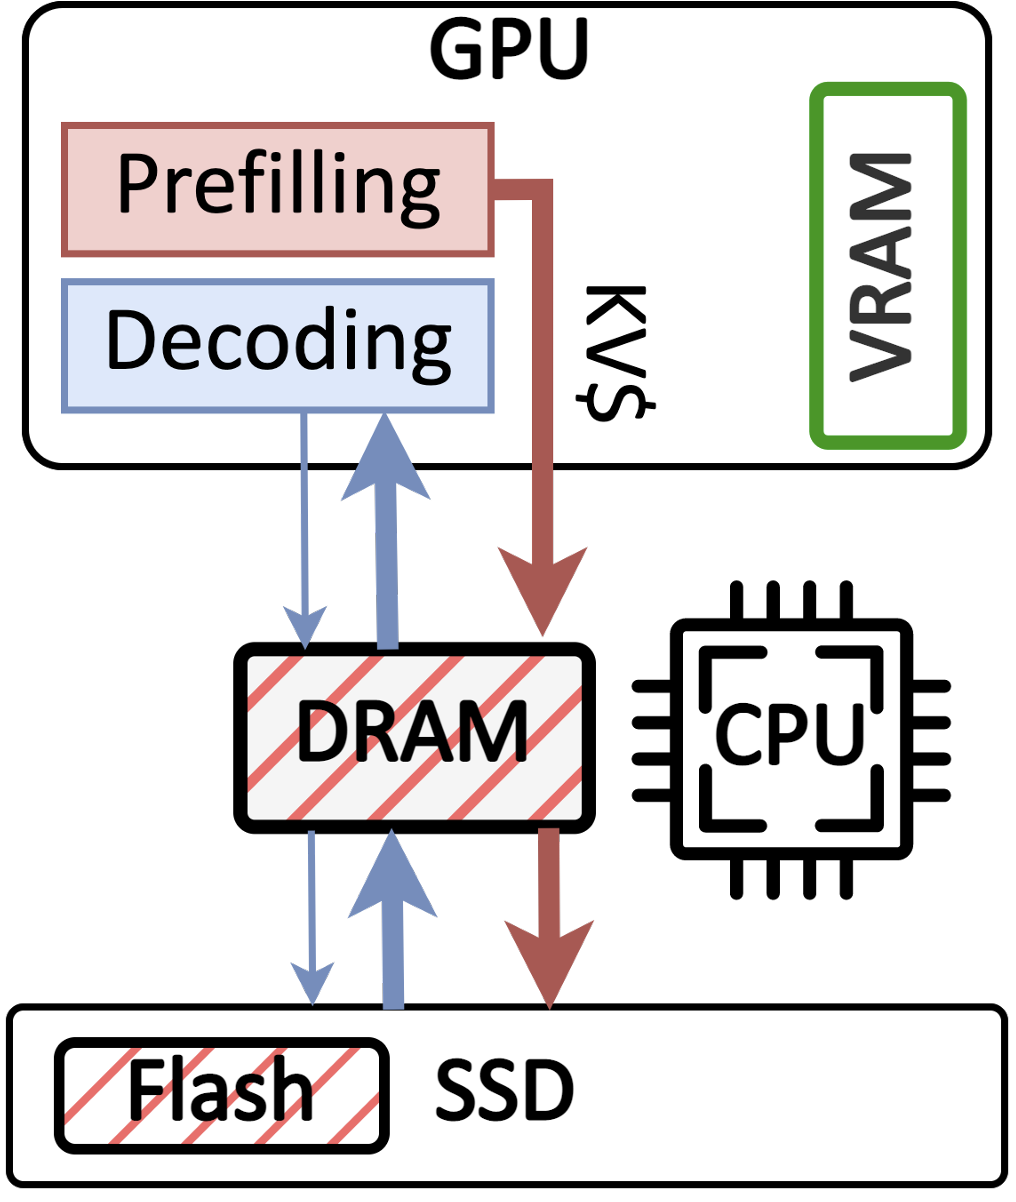
\includegraphics[width=0.22\textwidth]{figures/offloading.png}
    \caption{Offloading KV-cache to downstream memory tiers can improve the KV-cache capacity, but may introduce KV-cache transfer bottleneck over slow interconnect fabrics.}
    \label{fig:offloading}
\end{figure}


\subsection{Storage Hierarchy and Data Movement}\label{sec:techniques:movement}

\paragraph{Expanding capacity.}
A storage hierarchy combines devices with different capacities and access costs. \emph{Offloading} places data outside GPU memory to free space for active computation. FlexGen coordinates tensor placement and access across GPU memory, CPU memory, and disk~\cite{kv_sheng2023flexgen}. It also supports delegating attention computation to the CPU when avoiding cache transfers outweighs slower execution. These choices support larger batches under limited GPU capacity, but its throughput-oriented design can increase response time.

\paragraph{Selecting accesses without deleting history.}
Reducing the entries read at each step is distinct from permanently evicting them. QUEST uses the current query and per-channel minimum and maximum keys in each cache page to estimate page importance, then reads selected pages for attention~\cite{kv_tang2024quest}. Other pages remain available for later queries. This primarily relieves access bandwidth pressure rather than total storage demand, and introduces selection work and attention approximation. ShadowKV combines selective access with capacity reduction: it retains a low-rank key representation, offloads values, and reconstructs selected keys while fetching the corresponding values~\cite{kv_sun2025shadowkv}. Its benefit depends on balancing reduced transfers against selection, reconstruction, and approximation costs.

\paragraph{Co-design with sparse attention.}
HiSparse~\cite{kv_xie2026hisparse} connects sparse attention with hierarchical storage. Sparse attention selects only a subset of historical positions at each step, but future selections may still require the full history. HiSparse keeps this history in CPU memory and maps selected positions to a bounded set of GPU cache slots, fetching only missing entries. Compact state used to select positions remains on the GPU. For models that share selections across layers, later layers' accesses are known early, enabling prefetching during earlier computation. This is a co-design opportunity: model-level sharing exposes future accesses to the storage system. HiSparse changes placement without adding approximation to the underlying sparse attention; its costs are cache management and transfers on misses.

\paragraph{Reducing transfer overhead.}
InfiniGen predicts important KV entries for a subsequent layer and fetches them from CPU memory ahead of use, a technique called \emph{prefetching}~\cite{kv_lee2024infinigen}. Selective fetching reduces traffic and can overlap transfers with computation. It adds prediction work and may introduce attention error: entries omitted from a computation do not contribute to its output, even if they remain stored elsewhere. This connects access optimization with the selective methods in Section~\ref{sec:techniques:retention}.

\paragraph{Moving data or moving computation.}
NEO offloads part of both the cache and attention computation to the CPU~\cite{kv_jiang2025neo}. Processing entries where they reside avoids repeatedly transferring the full offloaded history. Its pipeline overlaps CPU and GPU work, while load-aware scheduling balances their responsibilities.

The central trade-off is between transferring KV data for GPU execution and computing near CPU-resident data. The former can be limited by transfer bandwidth; the latter reduces traffic but may bottleneck on CPU computation or memory bandwidth. Systems must balance these costs according to the volume of accessed data, hardware capabilities, and current load.

DirectKV uses fast links between CPUs and GPUs to change this access path~\cite{kv_luo2026directkv}. On platforms such as GH200, GPU attention routines directly read CPU-resident KV instead of first copying it into a GPU staging buffer. This saves temporary GPU capacity and avoids redundant movement, but still consumes interconnect bandwidth. It requires hardware and attention routines suited to direct CPU-memory access; zero-copy does not imply zero communication.

\paragraph{Encoding for network transfer.}
CacheGen reduces context-loading delay by encoding KV tensors into compact bitstreams and adapting compression levels to available network bandwidth~\cite{kv_liu2024cachegen}. Its objective differs from minimizing resident GPU cache size: encoding and decoding must be inexpensive enough that reduced transmission time produces a net benefit. Stronger compression can reduce preparation delay on a slow link while increasing approximation error. This connects representation choices to the conditions under which cached state is delivered.


\subsection{Comparison}\label{sec:techniques:storage-summary}

Table~\ref{tab:storage-comparison} summarizes the main benefits and costs. Allocation reduces wasted capacity; offloading expands available capacity; access optimization reduces traffic or waiting. These benefits are distinct: paging does not by itself reduce the historical entries required by dense attention, and a larger storage tier may increase state preparation time.

\begin{table}[tbp]
    \centering
    \caption{Representative storage and access mechanisms and their principal trade-offs. Benefits depend on the workload and hardware.}
    \label{tab:storage-comparison}
    \begingroup
    \footnotesize
    \setlength{\tabcolsep}{4pt}
    \renewcommand{\arraystretch}{1.15}
    \begin{tabularx}{\textwidth}{@{}>{\raggedright\arraybackslash}p{0.22\textwidth}>{\raggedright\arraybackslash}p{0.30\textwidth}>{\raggedright\arraybackslash}X@{}}
        \toprule
        \textbf{Method} & \textbf{Main benefit} & \textbf{Main cost or limitation} \\
        \midrule
        PagedAttention~\cite{kv_kwon2023pagedattention} & Less allocation waste & Block mappings; adapted attention kernels \\
        vAttention~\cite{kv_prabhu2025vattention} & Dynamic physical allocation & Virtual-memory mapping and allocation costs \\
        FlashInfer~\cite{kv_ye2025flashinfer} & Efficient access to varied layouts & Layout-specific attention support \\
        \addlinespace[4pt]
        FlexGen~\cite{kv_sheng2023flexgen} & Larger effective capacity & Transfers; latency-insensitive workload focus \\
        QUEST~\cite{kv_tang2024quest} & Fewer pages read per query & Selection; attention approximation \\
        HiSparse~\cite{kv_xie2026hisparse} & Bounded GPU KV residency & Sparse access required; miss transfers \\
        InfiniGen~\cite{kv_lee2024infinigen} & Less transfer traffic and waiting & Prediction overhead; attention approximation \\
        NEO~\cite{kv_jiang2025neo} & More capacity; less cache movement & CPU resource demand; pipeline balancing \\
        DirectKV~\cite{kv_luo2026directkv} & No GPU staging copy & Fast interconnect; adapted attention routines \\
        \addlinespace[4pt]
        CacheGen~\cite{kv_liu2024cachegen} & Less network traffic & Encoding cost; compression error \\
        \bottomrule
    \end{tabularx}
    \endgroup
\end{table}

These mechanisms complement compression when storage and attention support the chosen format. Reuse management determines which cached entries to retrieve or recompute.

\section{Reuse and Execution}\label{sec:techniques:reuse}

Reuse and execution management determines which requests can use existing KV-cache and how to coordinate their execution with cache availability. We organize these decisions around identifying reusable state, retaining it between requests, and assigning work to the resources that can use it. The main opportunity is to reduce state preparation overhead, while accounting for the capacity and bandwidth consumed by reuse.


\begin{figure}[h]
    \centering
    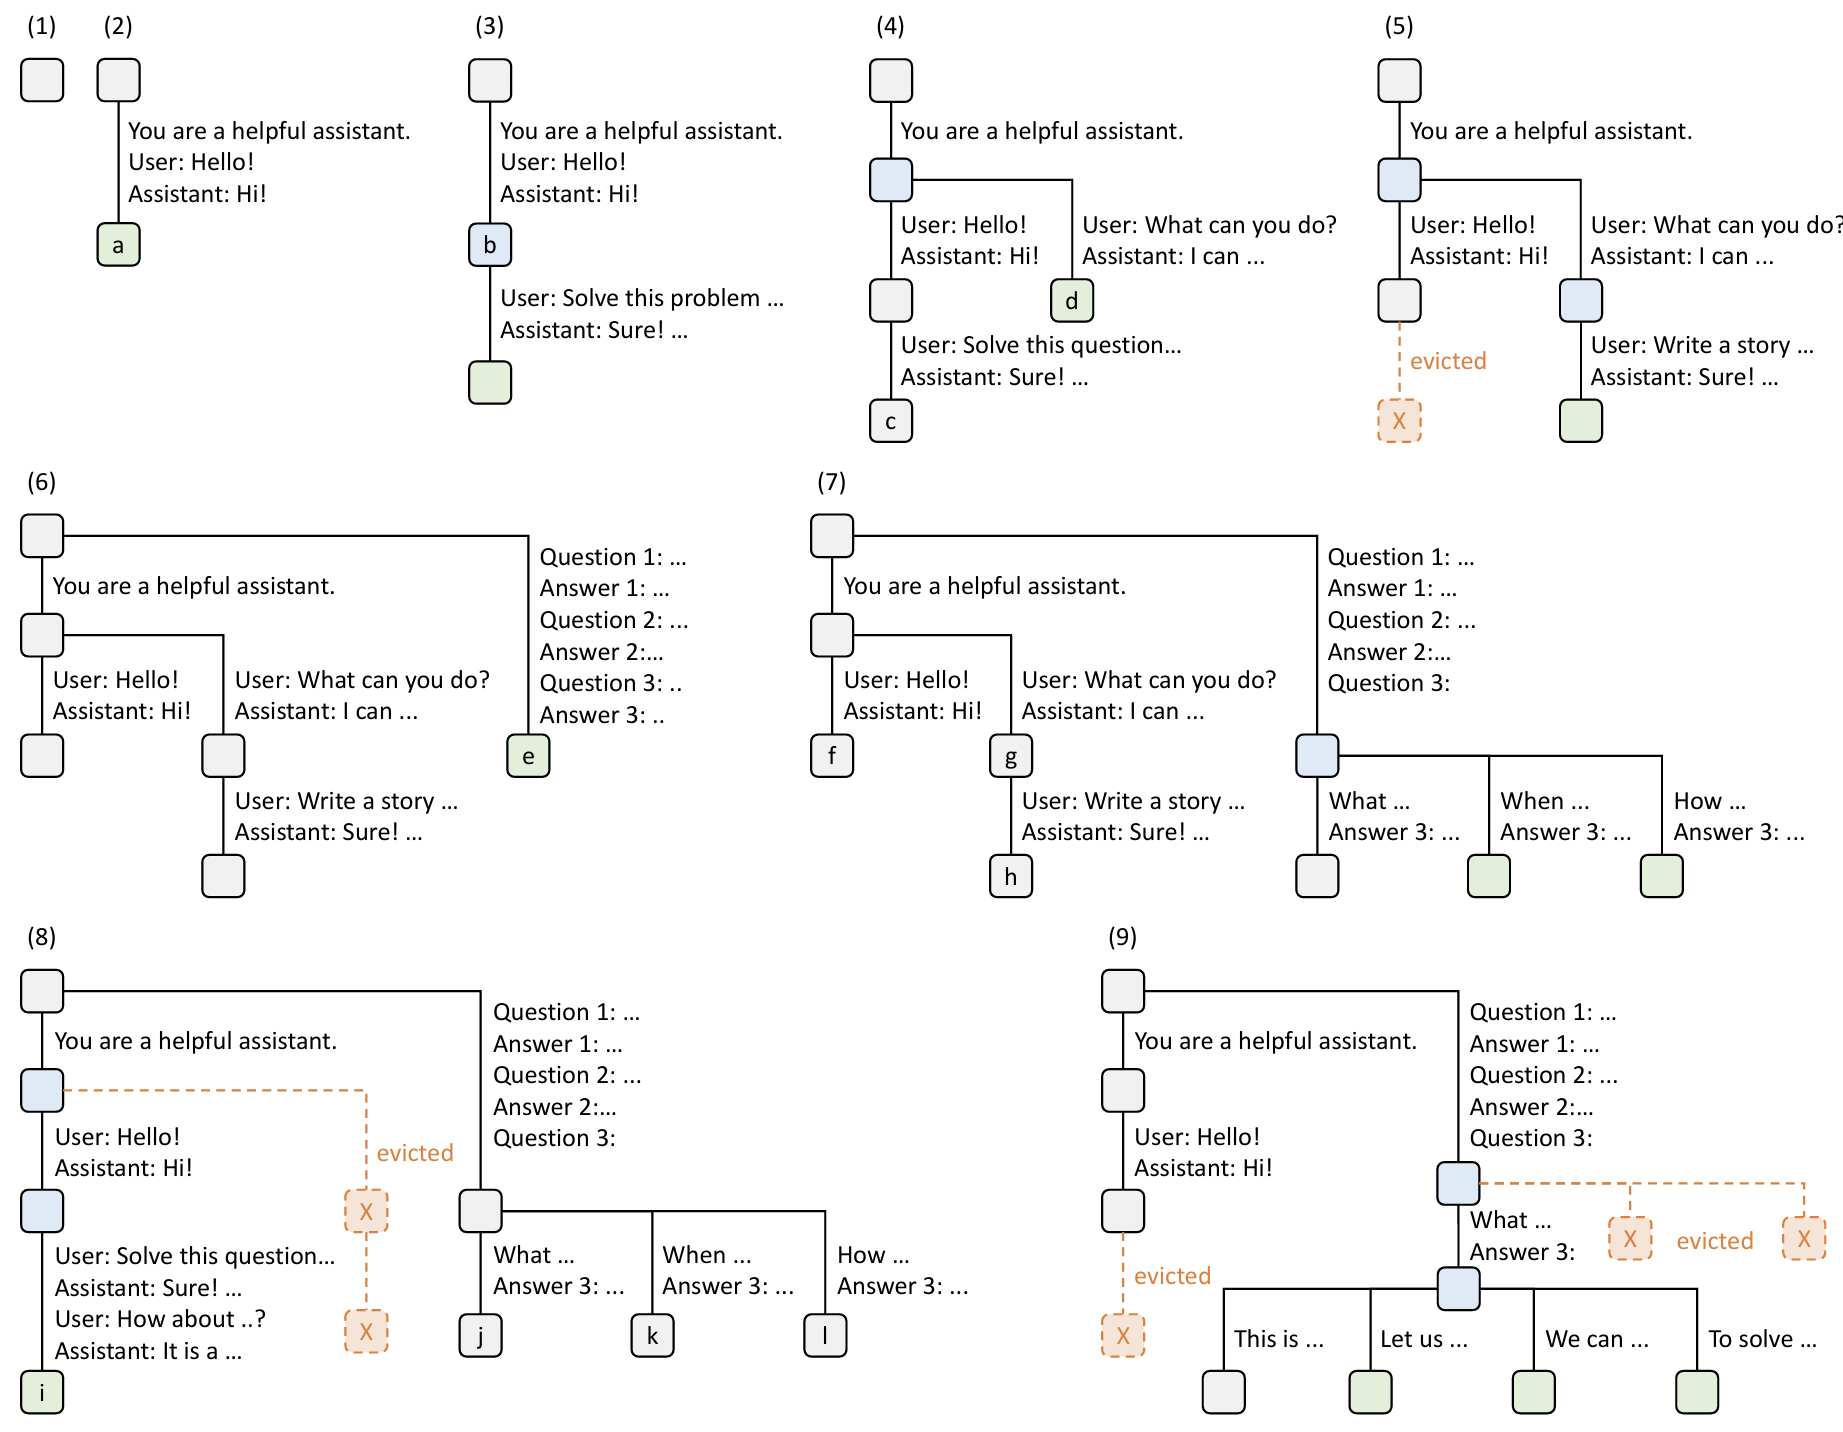
\includegraphics[width=0.9\textwidth]{figures/prefix.png}
    \caption{Prefix sharing through Radix Tree. Sharing KV-cache of the same segment of sequence can avoid re-prefill and save the memory space required for storing KV-cache.}
    \label{fig:prefix}
\end{figure}

\subsection{Reuse Scope and Matching}\label{sec:techniques:matching}

\paragraph{Matching common prefixes.}
Under causal attention, a prefix's KV-cache does not depend on tokens that follow it. Requests with the same token prefix can therefore reuse its cache, provided the model, token positions, and attention configuration are compatible. SGLang implements this reuse through RadixAttention~\cite{kv_zheng2024sglang}. It indexes token sequences in a \emph{radix tree}, a tree whose edges represent token segments and whose shared paths represent common prefixes. A new request follows these paths to find the longest cached prefix; only the remaining suffix requires prefill. This supports reuse across both concurrent requests and successive calls. Its scope is constrained by prefix identity: matching a passage that appears after a different preceding context is insufficient.

\paragraph{Reusing non-prefix passages.}
Document question answering often combines retrieved passages in different orders. Concatenating their independently computed KV-cache introduces two problems. First, \emph{positional encoding} must match the new input: cached keys may encode a passage's original token positions rather than its positions after concatenation, producing incorrect attention scores unless corrected. Second, \emph{causal dependencies in the attention forward pass} are missing. For an input consisting of passage $A$ followed by passage $B$, tokens in $B$ can attend to preceding tokens in $A$. Computing $B$ independently omits these interactions. Its attention outputs, and consequently the KV generated in subsequent layers, can therefore differ from full prefill of the combined input. Correcting positional encoding alone cannot reconstruct these missing computations.

CacheBlend observes that these dependencies affect tokens unevenly~\cite{kv_yao2025cacheblend}. It measures \emph{KV deviation}, the difference between cached and recomputed KV. Updating a small fraction of high-deviation tokens can preserve generation quality in its experiments. This supports approximate reuse: skipped entries may still contain errors, but their effects can be small enough to tolerate.

The design first corrects cached keys for all shifted tokens using rotary positional encoding (RoPE), which encodes position through vector rotations. It then progressively filters tokens for recomputation across layers. Starting with all tokens, it uses differences between newly computed and cached KV to select candidates for subsequent layers, exploiting the observed correlation of deviations across neighboring layers. Later filtering considers only the remaining candidates; it does not first obtain full-prefill KV for every layer. Selected tokens recompute their queries, keys, values, and layer outputs, while attending to a mixture of updated and cached KV at all causally visible positions. Savings come from skipping other tokens' computation in later layers. This trades state preparation work against selection overhead and approximation error, without guaranteeing equivalence to full prefill.

Prompt structure offers another way to organize reuse. Prompt Cache lets applications declare reusable modules and their positional arrangements through a schema~\cite{kv_gim2024promptcache}. This makes reuse explicit, but positional consistency alone does not reconstruct attention dependencies between independently prepared modules. CacheSlide targets agent prompts whose reusable segments preserve their relative order while shifting in absolute position~\cite{kv_liu2026cacheslide}. It combines a position-encoding scheme for these segments with partial attention computation and learned weights for mixing updated and cached KV. These methods exploit structured workloads to broaden reuse, with costs in application constraints, correction work, or learned configuration.

\subsection{Cache Retention and Restoration across Requests}\label{sec:techniques:cache-lifetime}

Completing a request does not necessarily end the usefulness of its cache. In a multi-turn conversation, the next request typically includes the previous interaction as a prefix. Keeping that state avoids rebuilding it, but competes with other cached contexts and active requests for capacity. Unlike removing tokens from an active sequence in Section~\ref{sec:techniques:retention}, evicting an inactive cache sacrifices a future reuse opportunity rather than directly approximating the current attention computation.

SGLang retains prefixes after requests finish~\cite{kv_zheng2024sglang}. To reclaim space, it removes the least recently used eligible leaves of its radix tree. Shared ancestors remain reusable, while references from running requests protect entries still in use. Recency provides an inexpensive retention rule, although it cannot predict all future accesses.

Pensieve and CachedAttention retain conversation state across turns rather than discarding it after each response~\cite{kv_yu2025pensieve,kv_gao2024cachedattention}. Pensieve manages history across GPU and CPU memory and supports attention over non-contiguous cached data. CachedAttention coordinates fetching and eviction with hints from the inference scheduler, prioritizing state required by upcoming requests. Layer-wise pre-loading and asynchronous saving overlap access with computation. Both reduce repeated prefill by extending cache lifetime, while retaining history consumes storage and makes restoration part of request latency.

HCache introduces an intermediate option between loading complete KV and recomputing from tokens~\cite{kv_gao2025hcache}. It saves the hidden states entering model layers and restores KV through their key and value projections, avoiding repeated attention and feed-forward computation. Its scheduler combines restoration methods to balance computation and I/O, while its storage organization reconciles incremental saving with bulk restoration. The capacity advantage depends on the model: hidden states need not be smaller than KV when few KV heads or latent representations are used. The broader principle is to choose both what state to retain and how to recover executable KV from it.

Retention should therefore consider both the likelihood of reuse and its cost. A large cache may save substantial prefill work but occupy space that could retain several other useful contexts. Similarly, finding a saved prefix is beneficial only when retrieving it is preferable to recomputing it under the current resource conditions. Cache hit rate alone does not capture this trade-off.

\paragraph{Sharing retained state across engines.}
LMCache makes retained KV reusable across requests and compatible inference engines through an independent cache-management layer~\cite{kv_liu2025lmcache}. Modular connectors let engines store and retrieve state from shared storage backends, while a control interface supports cache orchestration. The same layer also supports state handoff between prefill and decoding workers. This extends reuse beyond one engine's local cache, but requires compatible cache formats, model configurations, and attention settings. Retrieval and format-conversion costs still determine whether a cache hit saves preparation time.

\begin{figure}[h]
    \centering
    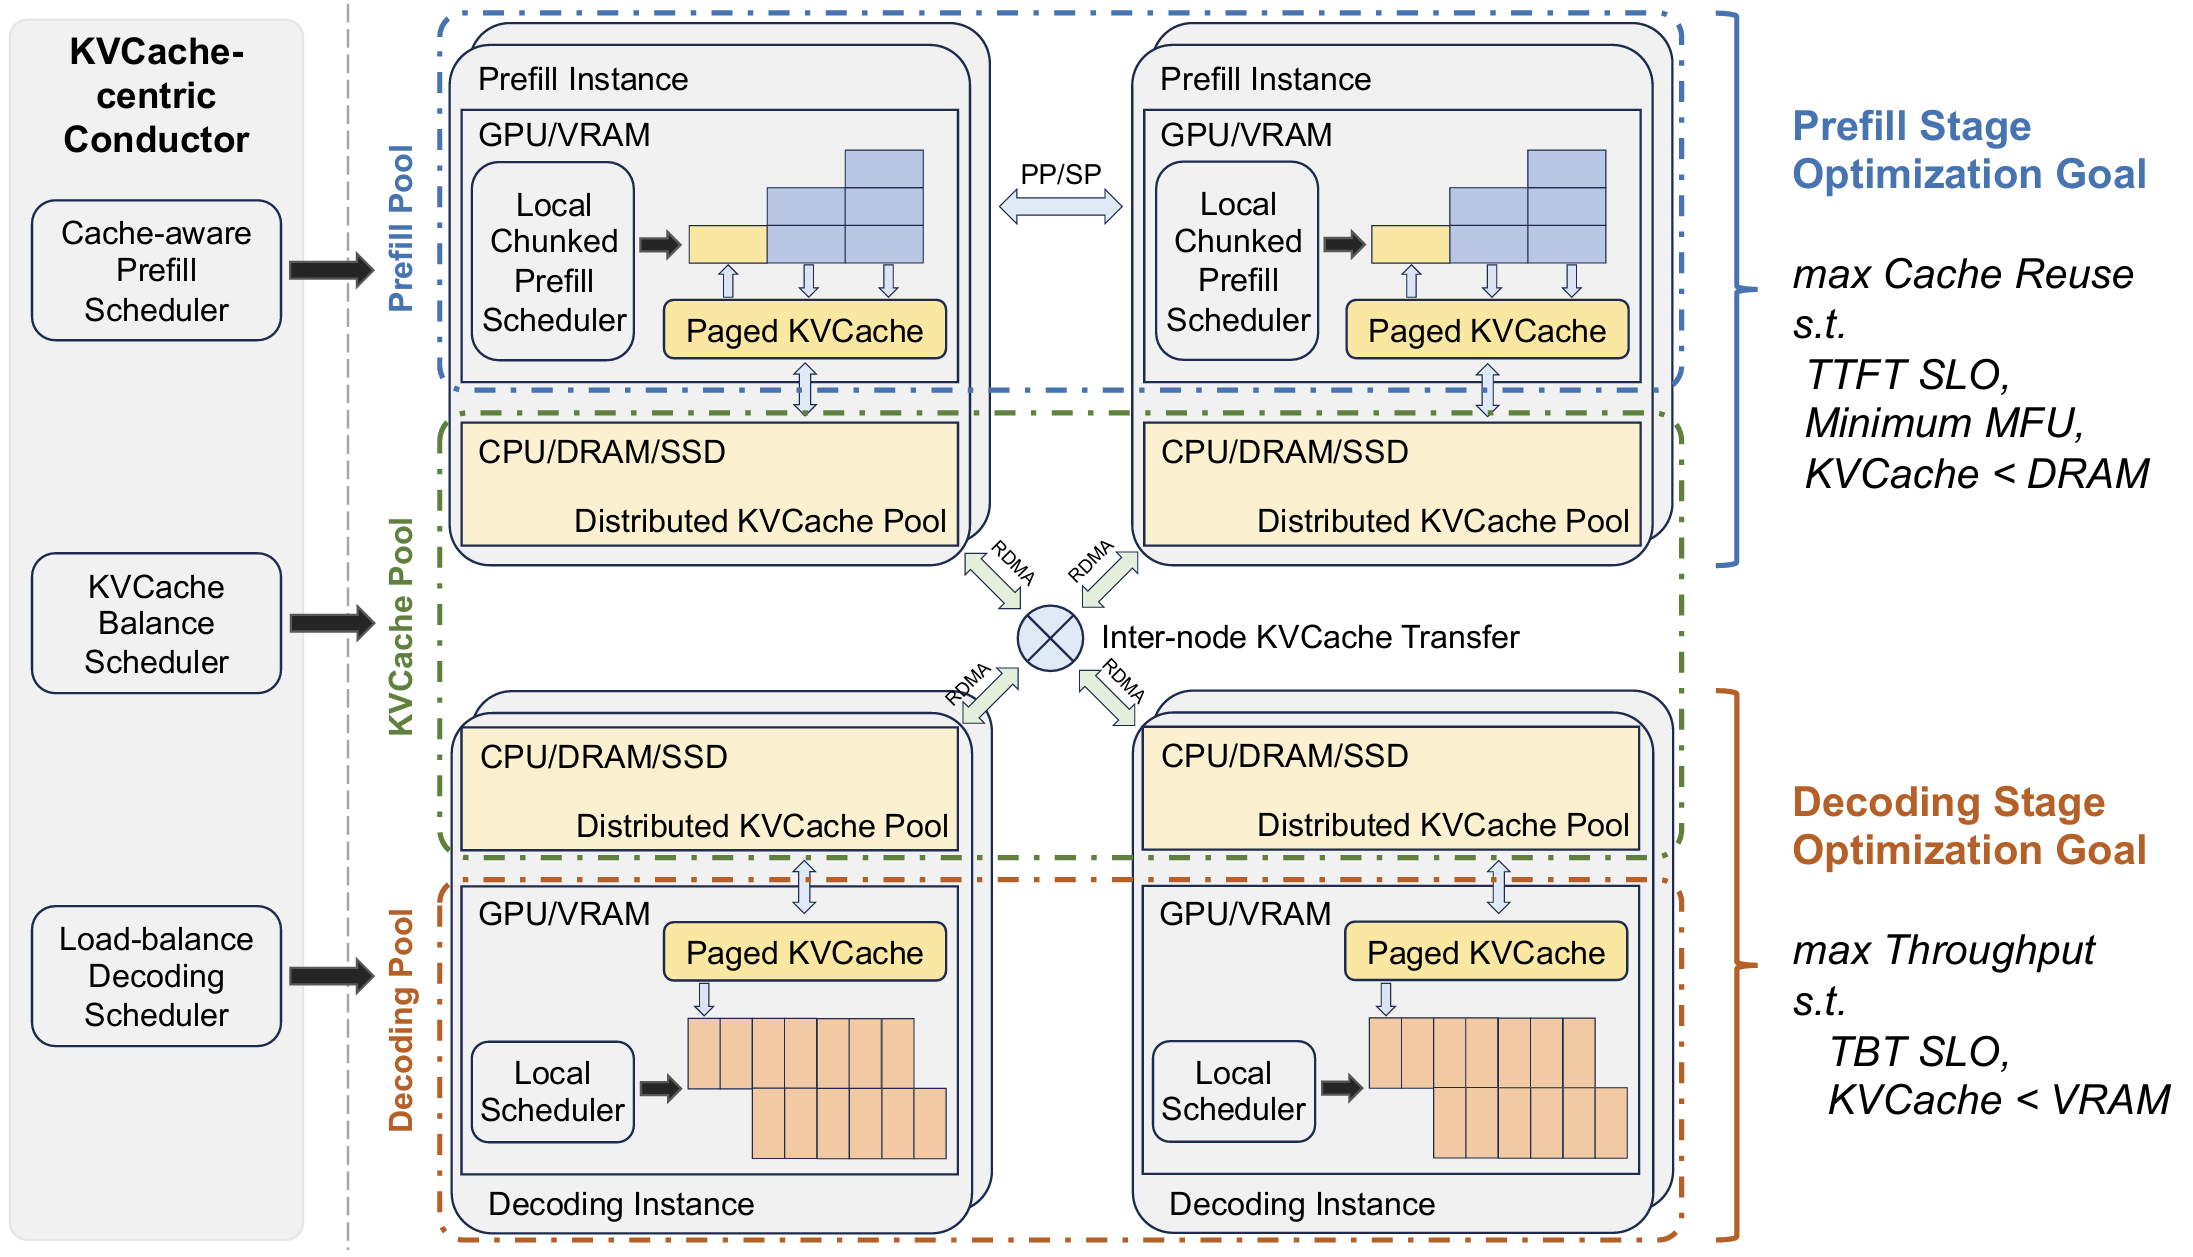
\includegraphics[width=0.9\textwidth]{figures/mooncake.png}
    \caption{The architecture of MoonCake. MoonCake maintains KV-cache pools on DRAM and SSD, retain KV-cache after request finished and reuse it when new request needs it. It also dynamically schedules and transfers KV-cache between GPU nodes.}
    \label{fig:mooncake}
\end{figure}

\subsection{Cache-aware Execution Coordination}\label{sec:techniques:coordination}

\paragraph{Assigning requests to servers.}
A server holding a useful prefix may also have a long request queue. Sending every matching request there can increase waiting time despite avoiding computation. Mooncake coordinates request assignment with its global KV-cache~\cite{kv_qin2025mooncake}. Its scheduler considers reusable prefix length, cache location, and server load when selecting a prefill instance. It can retrieve remote cached state or recompute tokens when transfer is less attractive. The decision therefore balances saved prefill work against queueing and data movement, rather than simply choosing the largest prefix match. Maintaining cache-location information and estimating execution costs add management overhead.

\paragraph{Coordinating cache loading and migration.}
Strata accounts for cache-loading latency when forming batches and overlaps loading with complementary computation~\cite{kv_xie2026strata}. It also handles requests that arrive while the same context is still being loaded, avoiding the assumption that every cache hit is immediately ready. Llumnix addresses changes after execution has begun: it migrates requests and their in-memory state between model instances to improve load balance and isolation~\cite{kv_sun2024llumnix}. Loading-aware scheduling reduces waiting for retained state; live migration relocates active state. Both must weigh the execution benefit against movement and coordination costs.

\paragraph{Coordinating prefill and decoding.}
KV-cache also connects stages within one request: prefill produces the state that decoding consumes. DistServe assigns these stages to different GPUs to remove their interference, choosing resource allocation and placement with latency requirements and communication bandwidth in mind~\cite{kv_zhong2024distserve}. Splitwise emphasizes matching each phase to suitable hardware, including heterogeneous machines, to balance throughput, cost, and power~\cite{kv_patel2024splitwise}. Both introduce a cache handoff before decoding, so separation benefits must outweigh communication and coordination costs. This is execution management within a request, independent of cross-request prefix reuse.

\subsection{Comparison}\label{sec:techniques:reuse-summary}

Table~\ref{tab:reuse-comparison} compares the principal decisions. These mechanisms can work together: prefix matching identifies reusable work, retention makes it available over time, and execution coordination determines where and when it is consumed.

\begin{table}[t]
    \centering
    \caption{Representative reuse and execution management techniques and their principal trade-offs. Stage separation and migration do not require cross-request reuse.}
    \label{tab:reuse-comparison}
    \begingroup
    \footnotesize
    \setlength{\tabcolsep}{4pt}
    \renewcommand{\arraystretch}{1.15}
    \begin{tabularx}{\textwidth}{@{}>{\raggedright\arraybackslash}p{0.25\textwidth}>{\raggedright\arraybackslash}p{0.32\textwidth}>{\raggedright\arraybackslash}X@{}}
        \toprule
        \textbf{Method} & \textbf{Main decision} & \textbf{Main cost or limitation} \\
        \midrule
        SGLang~\cite{kv_zheng2024sglang} & Match and retain shared prefixes & Prefix identity; retained capacity \\
        CacheBlend~\cite{kv_yao2025cacheblend} & Combine cached passages & Selective recomputation; quality risk \\
        Prompt Cache~\cite{kv_gim2024promptcache};\newline CacheSlide~\cite{kv_liu2026cacheslide} & Exploit structured prompt segments & Structural assumptions; context correction \\
        \addlinespace[4pt]
        Pensieve~\cite{kv_yu2025pensieve};\newline CachedAttention~\cite{kv_gao2024cachedattention} & Retain conversation state & Storage occupancy; restoration delay \\
        HCache~\cite{kv_gao2025hcache} & Restore KV from hidden states & Projection work; model-dependent size benefit \\
        LMCache~\cite{kv_liu2025lmcache} & Share retained state across requests and engines & Compatibility; retrieval and conversion costs \\
        \addlinespace[4pt]
        Mooncake~\cite{kv_qin2025mooncake} & Assign requests using cache and load information & Transfer cost; load estimation \\
        Strata~\cite{kv_xie2026strata};\newline Llumnix~\cite{kv_sun2024llumnix} & Coordinate loading or relocate active state & Movement and scheduling overhead \\
        DistServe~\cite{kv_zhong2024distserve};\newline Splitwise~\cite{kv_patel2024splitwise} & Place prefill and decoding separately & KV handoff; stage coordination \\
        \bottomrule
    \end{tabularx}
    \endgroup
\end{table}

Across the three challenges, these techniques primarily reduce repeated state generation or coordinate state availability with execution. Retention increases capacity demand, and restoration consumes bandwidth; approximate passage reuse adds computation and potential quality loss. The useful outcome is the preparation work and waiting time actually avoided, not the amount of cached data or the number of cache hits alone.
